\documentclass[10pt,a4paper]{article}

\usepackage[utf8]{inputenc}
\usepackage[francais]{babel}
\usepackage[T1]{fontenc}
\usepackage{amsmath}
\usepackage{amsfonts}
\usepackage{amssymb}
\usepackage{graphicx}
\usepackage{lmodern}
\usepackage{hyperref}
\usepackage[left=2.7cm,right=2.7cm,top=2cm,bottom=3cm]{geometry}
\usepackage{verbatim}
\usepackage{xcolor}
\usepackage{url}

\hypersetup{
    colorlinks,
    linkcolor={red!50!black},
    citecolor={blue!50!black},
    urlcolor={blue!80!black}
}

\title{
\includegraphics[scale=1]{Art/otb-logo.png}\\
  Guide d'installation OTB\\
  {\small\url{https://www.orfeo-toolbox.org}}
}

\begin{document}

\maketitle

\tableofcontents

\clearpage
\section{Windows}

\subsection{QGIS}
Installer QGIS: \url{http://www.qgis.org/fr/site/forusers/download.html}.
\subsection{Ligne de commande}
Installer un environnement minimal de ligne de commande pour Windows. Par exemple
Git for Windows est très facile à installer:
\url{http://git-scm.com/download/win}.

\subsection{OTB et Monteverdi}
Pour installer OTB 5.2.1 et Monteverdi 3.0.1, télécharger les paquets
correspondants à votre architecture (32 ou 64 bits). Si votre machine est 32
bits:

\begin{verbatim}
Monteverdi-3.0.1-win32.zip
OTB-5.2.1-win32.zip
\end{verbatim}

Sinon si votre machine est 64 bits:

\begin{verbatim}
Monteverdi-3.0.1-win64.zip
OTB-5.2.1-win64.zip
\end{verbatim}

Ces archives sont disponibles sur \url{https://www.orfeo-toolbox.org/packages/}.
Extraire les deux archives zip dans votre répertoire personnel, par exemple dans:\\
\begin{centering}
\texttt{C:{\textbackslash}Utilisateurs{\textbackslash}Martin{\textbackslash}install{\textbackslash}}.
\end{centering}

\subsection{Tester l'installation}
Une fois l'installation terminée, les applications OTB sont accessibles de
plusieurs façons. Verifier que l'installation est fonctionelle avec les étapes
suivantes:
\begin{enumerate}

\item Lancer monteverdi en navigant dans le dossier \texttt{bin} de son répertoire
d'installation, par exemple:
\texttt{Martin{\textbackslash}install{\textbackslash}Monteverdi-3.0.1-win32{\textbackslash}bin},
puis double cliquer sur \textbf{\texttt{monteverdi.bat}} (et non pas
\texttt{monteverdi.exe}).

\item Essayer d'ouvrir une image tif avec Monteverdi (voir
  figure~\ref{fig:monteverdi}). Une image tif de démo est
disponible ici: \url{https://git.orfeo-toolbox.org/otb-data.git/blob/HEAD:/Examples/QB\_Toulouse\_Ortho\_PAN.tif}.

\item Charger les applications OTB avec "Fichier" $\rightarrow$ "Charger les
OTB-Applications".
Le navigateur d'application est ensuite accessible depuis "Affichage"
$\rightarrow$ "Navigateur d'OTB-Applications".
(Voir figure \ref{fig:windows-mapla}).

\item Naviguer dans le dossier \texttt{bin} du répertoire d'installation OTB et double cliquer sur le
fichier \texttt{.bat} de l'application à lancer, par exemple:\\
\texttt{Martin{\textbackslash}install{\textbackslash}OTB-5.2.1-win32{\textbackslash}bin{\textbackslash}otbgui\_Rescale.bat}
(Voir figure \ref{fig:windows-otbgui}).

\end{enumerate}

\begin{figure}[h]
  \center
  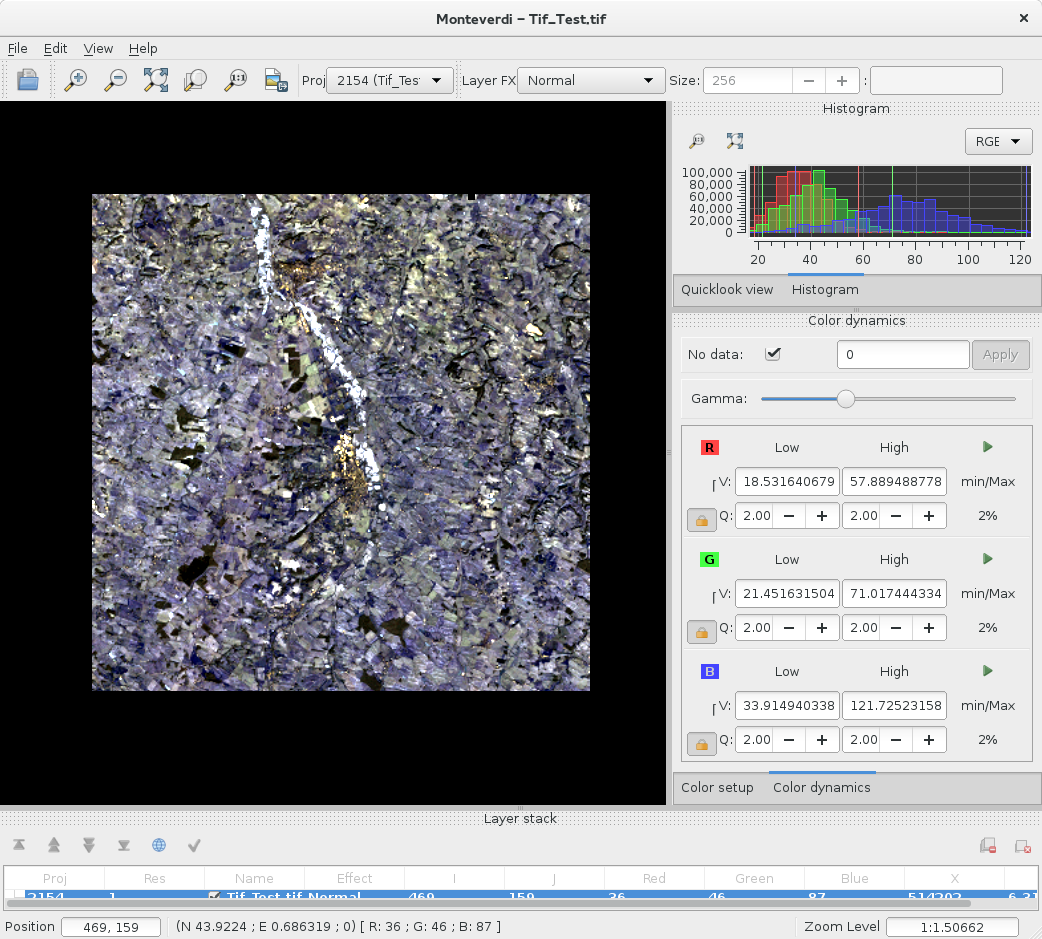
\includegraphics[width=1\textwidth]{Art/monteverdi-tif.png}
  \caption[]{Monteverdi}
  \label{fig:monteverdi}
\end{figure}

\begin{figure}[h]
  \center
  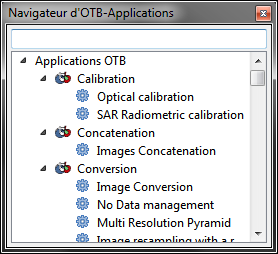
\includegraphics[scale=1]{Art/windows-mapla.png}
  \caption[]{Les applications OTB sont accessibles depuis Monteverdi}
  \label{fig:windows-mapla}
\end{figure}

\begin{figure}[h]
  \center
  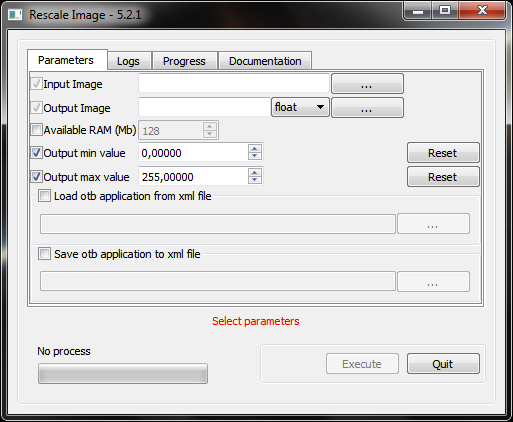
\includegraphics[scale=1]{Art/windows-otbgui.png}
  \caption[]{Interface graphique OTB}
  \label{fig:windows-otbgui}
\end{figure}

% En commentaire pour l'instant, c'est peut être un peu inutile puisqu'il n'y a
% aucune action associée en terme d'installation
\begin{comment}
\subsection{OTB depuis QGIS}

Les applications OTB sont disponibles depuis QGIS. Pour cela

Attention ! QGIS est livré avec ses propres binaires OTB. Les applications ainsi
ouvertes depuis QGIS sont souvent différentes de celles installée ci-dessus, car
il s'agit typiquement d'une version plus ancienne.
Éventuellement, il est possible de remplacer l'OTB livrée avec QGIS en supprimant
ou écrasant les fichiers dans \texttt{}.

\begin{figure}[h]
  \center
  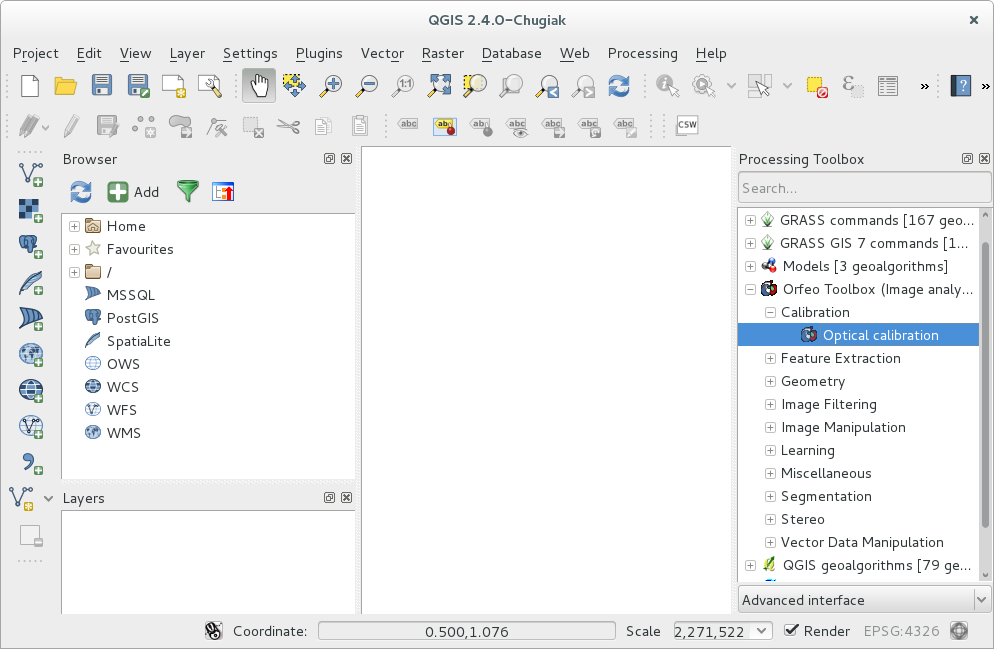
\includegraphics[width=1\textwidth]{Art/qgis-otb.png}
  \caption[]{Intégration QGIS - OTB}
  \label{fig:otb-qgis}
\end{figure}
\end{comment}

\clearpage
\section{Ubuntu}

\subsection{QGis}
QGis peut être installé via un gestionnaire de paquets graphique ou bien en 
ligne de commande, le paquet à installer s'appelle simplement \textbf{qgis}.
\begin{verbatim}
sudo apt-get install qgis
\end{verbatim}

\subsection{Installer les dépendences}
Avant d'installer le paquet autoportant OTB, certaines dépendences système
sont nécéssaires. Dans un terminal, taper:
\begin{verbatim}
sudo apt-get install libx11-6 libxext6 libxau6 libxxf86vm1 libxdmcp6 libdrm2
\end{verbatim}

Vous aurez en outre besoin des librairies libgl1 et libglu1, qui ont 
différentes implémentations (MESA, FGLRX, NVIDIA, ...). Si vous n'avez pas 
déjà ces librairies sur votre système, vous pouvez prendre une implémentation
libre comme MESA :
\begin{verbatim}
sudo apt-get install libgl1-mesa-glx libglu1-mesa
\end{verbatim}

\subsection{Installer OTB et Monteverdi}
Télécharger le paquet autoportant OTB pour linux (64 bits), disponible ici:
\begin{center}
\url{https://www.orfeo-toolbox.org/packages/OTB-5.2.1-Linux64.run}
\end{center}

Il s'agit d'une archive auto-extractible, qui va se déployer dans le répertoire
courant. Une fois rendue exécutable, l'archive peut être extraite. Les 
exécutables sont dans le sous-dossier 'bin', vous pouvez les rendre facilement
accessible en ajoutant ce chemin au PATH. Les commandes permettant de faire 
ce déployement sont :
\begin{verbatim}
chmod +x OTB-5.2.1-Linux64.run
./OTB-5.2.1-Linux64.run
export PATH=$PATH:<votre-répertoire-OTB>/bin
\end{verbatim}

Ensuite, il y a quelques variables d'environnement nécessaire pour bénéficier de 
toutes les fonctionnalités :
\begin{verbatim}
export GDAL_DATA=<votre-répertoire-OTB>/share/gdal
export OTB_APPLICATION_PATH=<votre-répertoire-OTB>/lib/otb/applications
\end{verbatim}

Note: lorsque vous renseignez des chemins dans des variables d'environnement,
utilisez des chemins absolus.

\subsection{Tester l'installation}
Une fois l'installation terminée, les applications OTB sont accessibles de
plusieurs façons. Verifier que l'installation est fonctionelle avec les étapes
suivantes:
\begin{enumerate}

\item Lancer Monteverdi (taper "monteverdi" dans un terminal) et essayer
d'ouvrir une image tif (voir figure~\ref{fig:monteverdi}). Une image tif de
démo est disponible ici:
\url{https://git.orfeo-toolbox.org/otb-data.git/blob/HEAD:/Examples/QB\_Toulouse\_Ortho\_PAN.tif}.

\item Charger les applications OTB avec "Fichier" $\rightarrow$ "Charger les
OTB-Applications".
Le navigateur d'application est ensuite accessible depuis "Affichage"
$\rightarrow$ "Navigateur d'OTB-Applications".
(Voir figure \ref{fig:windows-mapla}).

\item Ouvrir une application OTB via un terminal, par exemple
\texttt{otbgui\_Rescale}. (Voir figure \ref{fig:windows-otbgui}).

\end{enumerate}

\end{document}
